%!TEX root = ../thesis.tex
%*******************************************************************************
%****************************** Second Chapter *********************************
%*******************************************************************************
\chapter{Theory and State Of The Art}
\label{chapter:SOTA}
% \hspace{0,5cm}

The state of the art, for several years now, has been models based on transformers-type architecture \citep{DBLP:journals/corr/VaswaniSPUJGKP17} that achieve the best performance in natural language understanding, representation and generation. This chapter will briefly review the main architectures and models present in the state of the art, introduce the main techniques for post-training processes regarding the adaptation of models to human preferences and specific tasks, and finally, an introduction to the topic of interpretability of the models themselves.

\section {Transformer models} 

Language models are statistical models that aim to represent natural language. Their purpose is to generate a probability of a set of words based on large amounts of text. 
Since the emergence of early language models based on recurrent neural networks, long short-term memory, and so on, networks based on a transformers-type architecture have quickly caught on in this field, leading to innovative results in terms of performance on multitasking. Specifically, these models are based on the attention mechanism, which enables the models to learn better from the context they are enabled to read.
Their first advantage, starts from a computational assumption. Previous state-of-the-art networks, based, for example, on recurrent neural networks, had a large number of sequential operations within them, which inevitably led to slowness in terms of training and inference given the large amount of steps to be performed for both phases. For this reason, the proposed new self-attention mechanism has as its primary goal the presence of parallelizable operations, that is, independent of each other that can be solved in parallel, decreasing the computational load and especially the queue of operations to be performed.

Transformer networks, in their general architecture, are encoder-decoder networks \citep{cho-etal-2014-learning}, or sequence-to-sequence models that aim to obtain a reduced internal representation of the same proposed input and output. This representation, in the case of natural language, coincides with the concept of contest. By learning this representation, the models are able to understand the meaning of a given sequence of words (or tokens) without the meaning being explained in any way.

Specifically, having an input sequence $x = (x_1, ..., x_n)$ the purpose of the model will be to represent, in vector form, the sequence given as input in a reduced dimension $z = (z_1, ..., z_m)$. This operation is carried out by the encoding part of the model, which produces an encoding vector, which will then be passed to the decoding component that will generate an output only based on the $z$ representation, that is, a sequence $y = (y_1, ..., y_m)$. The  $y$ sequence is generated following an auto-regressive approach where, at each instant $t \in [1, m]$,  the model will look at all the previously seen symbols, so at all steps $\leq t - 1$.

\begin{figure}
    \centering
    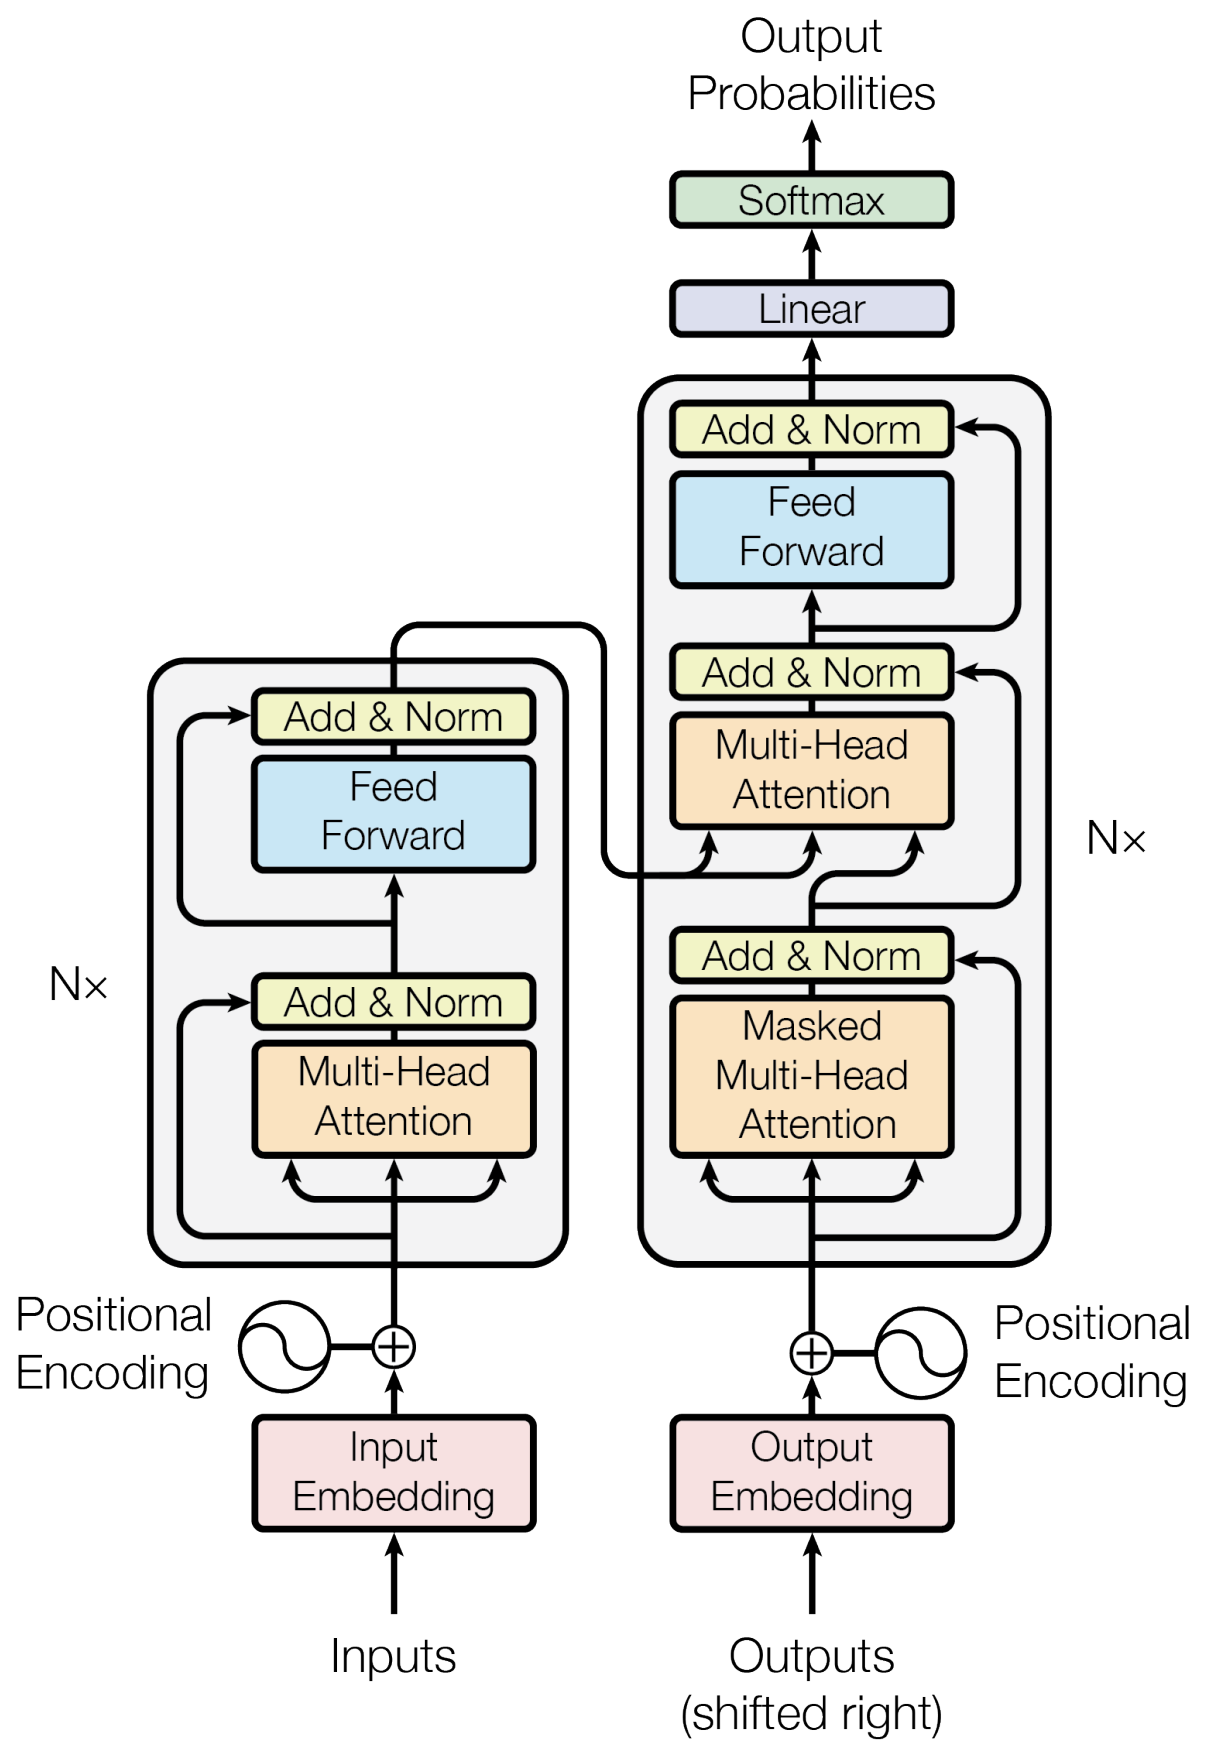
\includegraphics[width=0.4\linewidth]{Figs/transformer.png}
    \caption{The Transformer - model architecture from \citep{DBLP:journals/corr/VaswaniSPUJGKP17}}.
    \label{fig:transformers-arch}
\end{figure}

By looking at the transformer architecture in Figure \ref{fig:transformers-arch} the general model makes use of several blocks throughout the encoder and decoder, like point-wise and fully connected layers. Specifically, both the encoder and the decoder (left and right sides respectively) are composed of a series of overlapping identical layers. The number of these layers, together with their elements, establishes the size of the model and particularly influences the number of parameters it contains. 

Each layer contains several components within it. The first element is the self-attention mechanism, then follows a fully connected feed-forward network. It is important to note that there are residual connections after each sub-layer of the architecture followed by normalization. Specifically, any output from the previous layer is both propagated to the next layer and preserved in its original form in the following way: $\text{LayerNorm}(x + \text{Sublayer}(x))$ where $\text{Sublayer}(x)$ is any type of function from the sublayer itself. As expected, the decoder takes the input from the encoder part of the architecture, implementing the same characteristics observed for the encoder with self-attention, residual connection and Layer Normalization.

An important factor that allows this type of model to outperform any other current neural network architecture is the presence of the self-attention mechanism. Given the input embedding matrix $X$, the self-attention modules multiply it with three weight matrices $W^Q, W^K, W^V$ respectively for queries, keys and values. Those are combined together by the scaled dot-product self-attention as follows:

\begin{equation*}
    \text{Attention} (Q, K, V) = \text{softmax} \left ( \frac{QK^T}{\sqrt{d_k}} \right )
\end{equation*}

where $d_k$ is the shape of the query and keys vectors used as scaling factor for stability purposes. Moreover, this mechanism is repeated in parallel $h$ times, and considering $L$ as the number of total layers stacked together, the total number of attention mechanisms in transformer architecture is $L \times h$. The purpose of using this parallelism, in addition to better computational scalability, is to combine multiple potentially different representations from multiple locations in the text. Given multiple single heads of attention it is possible to achieve:  

\begin{equation*}
    \text{MultiHead} (Q, K, V) = \text{Concat} (\text{head}_1, ..., \text{head}_h) W^O
\end{equation*}

where each head is defined as:

\begin{equation*}
    \text{head}_i = \text{Attention} (QW^{Q}_{i}, KW^{K}_{i}, VW^{V}_{i})
\end{equation*}

As already anticipated, the reasons why this architecture outperforms what has been seen in NLP in the past stem mainly from two factors. 

The first is definitely the scalability of self-attention-based networks, as they are extremely parallelizable and therefore excellent for the computation performed by modern GPUs capable of performing simple computations simultaneously. The advantage of quickly scaling the number of parameters is a feature that will be addressed later in the next chapters along with all the limitations that arise with this feature. 

The second reason lies in the inherent operation of this architecture. In fact, the self-attention mechanism allows for the best representation of the text taken as input, not neglecting the long-range dependencies that were previously difficult to capture, e.g. by recurrent-type networks. The internal attention matrix makes it possible to compare any token in a sentence with any other token regardless of their mutual position and thus their distance. This allowed a representation of the context of the sentence, and thus an understanding of it, that was previously hardly achieved by the state of the art in natural language understanding.


\section {Generative Language Models} 

The language modelling (LM) task is one of the major approaches now used to enable machines to understand natural language. In general, LMs aim to model the generative likelihood of word sequences, so as to predict the probabilities of feature tokens \citep{zhao2023survey}. Formally, let $(y_1, y_2, ..., y_n)$ be tokens in a text corpus (or sentence for simplicity), and $P(y_1, y_2, ..., y_n)$ the probability to see all these tokens following this specific order. By using the chain rule for probability, it is possible to derive the following product:

\begin{equation*}
    P(y_1, y_2, ..., y_n) = P(y_1) \cdot P(y_2 | y_1) \cdot P(y_3 | y_1, y_2) \cdot ... \cdot P(y_n | y_1, ..., y_{n-1}) = \prod_{t = 1}^n P(y_t | y_{<t}) 
\end{equation*}

also defined as a left-to-right language modelling framework, used by most of the generative language models.

Generation is handled differently according to the cases of interest. As anticipated, the next token is taken by considering the probability distribution over the entire vocabulary conditioned on the presence of all previous tokens:

\begin{equation*}
    y_t = \text{argmax}_y \prod_{t=1}^t (P(y | y_{<t - 1}))
\end{equation*}

This technique is defined as greedy search, i.e. selecting the highest probability token at each step. A more widely used approach is called beam search, where multiple candidates (called beams) are considered at each step:

\begin{equation*}
    y_t = \text{argmax}_y \prod_{t=1}^t (P(y^k | y_{<t - 1}))
\end{equation*}

or using log probability:

\begin{equation*}
    y_t = \text{argmax}_y \sum_{t=1}^t \log (P(y^k | y_{<t - 1}))
\end{equation*}

with any $k$-th token in a beam. The advantage of this technique is to select a less constrained generation, and thus an output more similar to human language. Generally, these techniques are combined with parameters such as temperature, top probability (only candidates with a probability above a certain threshold are considered) or top token (a maximum number of tokens to be considered per beam search is imposed).

Pre-trained Language Models, introduced for the first time with ELMo \citep{peters-etal-2018-deep}, were proposed to capture context-aware word representations by pre-training a Bi-LSTM network on a large text corpus and then fine-tuning it according to any specific downstream task. As previously mentioned, after the introduction of Transformers network \citep{DBLP:journals/corr/VaswaniSPUJGKP17} the highly parallelizable and the great learning capabilities of the architecture unlocked new state-of-the-art performance in the area of natural language understanding and representation. BERT \citep{devlin-etal-2019-bert} is one of the first attempts in this regard, achieving never-seen performance on a huge amount of NLP tasks.

Since then, researchers have found that by scaling parameters, better performance could be achieved, both in terms of language representation and generation itself \citep{kaplan2020scaling}. There is a correlation in this regard in terms of the number of parameters and size of datasets that can be used in the pre-training phase, and consequently to the computational power available. These three aspects, directly proportioned, can increase the performance of the models by absolutely guaranteeing their scalability. In addition, the larger the model, the higher its efficiency in terms of data points needed for convergence for further optimization applicable after the pre-training process.


New models, such as 175B-parameters GPT-3 from \citet{brown2020language} (or the most recent GPT-4 from \citet{openai2023gpt4}), 540B-parameters PaLM from \citet{chowdhery2022palm} and LLaMA 2 from \citet{touvron2023llama} showed not only great performances, beating the SOTA for that time, but also enabled new discoveries defined as \textit{emergent-abilities} \citep{wei2022emergent} for solving new and complex task (e.g. reasoning and solving problems expressed in natural language) behaving as few shot learners. A remarkable application of Large-LMs (LLMs) is ChatGPT \footnote{\href{https://openai.com/blog/chatgpt/}{\texttt{openai.com/blog/chatgpt/}}}, where a LLM is adapted to dialogue with the user showing great conversation capabilities with humans.


Experimentally, it has been possible to demonstrate how LLMs are able to achieve different abilities that exceed the random threshold in terms of performance. A non-exhaustive list may include:
\begin{itemize}
    \item \textbf{In-context learning}: the ability of LLMs to learn for examples in the input and provide a solution to a problem just by generating the expected output. This process happens without updating the parameters and further training the model for a specific task. This performance was first observed in GPT-3 \citep{brown2020language} and works well even for strict non-language tasks such as arithmetic tasks.
    \item \textbf{Instruction following} (or tuning): by fine-tuning a LLM with a collection of various NLP tasks (e.g. Question-Answering) it is possible to improve model reasoning performance for seen and unseen tasks described in the form of instructions \citep{NEURIPS2022_b1efde53, sanh2022multitask, wei2022finetuned}.
    \item \textbf{Step-by-step reasoning}: by using chain-of-thought (CoT) prompting strategy \citep{wei2023chainofthought} it is possible to solve complex problems by breaking them down into multiple steps that can be easily solved by the model itself. This approach also allows the model to consider the previous problem step just solved as input, enabling it to reason more effectively during the course of text generation.
\end{itemize}

\subsection{General issues concerning LLMs}

\paragraph{Utilization of LLMs} As mentioned, LLMs, in addition to their excellent performance, bring with them a number of necessary issues to mention. Certainly, there is an issue of computational power to be able to operate these models; the aforementioned ChatGPT (thus all the latest variants of GPTs) or all the other open-source and non-open-source models, with their billions of parameters, require not inconsiderable computational resources. Almost all of the computational load is handled by graphics cards and their memory, which are capable, respectively, of performing the necessary calculations (which usually are parallelizable matrix multiplications) and keeping a large amount of associated parameters in memory. Despite the progress of the semiconductor engineering industry, it is still very difficult to be able to pre-train (or even infer) without having computational clusters costing millions. 

To provide a concrete example of the pre-training of a LLM, BLOOM \citep{workshop2023bloom} is a 176-billion-parameter model trained by BigScience, a cooperative organization among several institutions and companies in the research and AI field. The training process has been made completely open-source, giving the ability to look at both the techniques and the amount of time and resources spent training the model. Specifically, the pre-training process employed a total of 384 Nvidia A100 80GB GPUs distributed across 48 nodes (416 of the same GPUs over 52 nodes if we include the backup system), each equipped with top-tier CPUs and half a terabyte of RAM. The dataset includes a total of 46 different languages for an occupied space of nearly 2TB. A single training epoch (i.e., a single pass over the entire dataset) took 3.5 months H24 to complete, with several backup infrastructures for failures due to the hardware employed. The total cost is estimated to be between $2-5$\$ millions just and exclusively for computational resources and cloud computing, thus excluding costs related to training set-up time and all personnel involved.

For this reason, the vast majority of these models are the exclusive preserve of the largest technology companies, the only ones who can currently afford this kind of cost. However, new solutions are constantly emerging in research that allows these models to be used on \textit{prosumer hardware} as well, i.e. hardware that is certainly high in cost but more accessible to the researcher market. This will be addressed in a later chapter (\ref{chapter:model-scale}) regarding the research project under discussion.

Other issues, which can be directly linked to the size of the models, include their environmental impact in terms of resources used (i.e., energy and materials used in their realization and deployment process, \citep{strubell-etal-2019-energy}), as well as their democratization in terms of access to people from all over the world, both in terms of technological and linguistic availability.

\paragraph{Data used for pre-training a LLM} The importance of data, especially in the presence of billions of parameters, is fundamental to pre-train an effective LLM \citep{hoffmann2022training}. To develop a capable LLM a large amount of natural language corpus from various data sources is needed. Usually, existing LLMs mainly leverage a mixture of diverse public textual datasets. Most of the data comes from web pages, books and conversational text helping the model to generalize better and grasp patterns from natural language in various styles and scenarios. In some cases pre-train corpus supplements the original data with scientific corpus, code, and task-dependent data \citep{chowdhery2022palm, zhang2022opt}. Especially in data collected from the Web, control is often applied automatically by different types of filters, but these do not always succeed in capturing only quality text. In addition to popular vetted sources, such as Wikipedia, low-quality text, spam or content from questionable sites are also included in datasets, eventually expanding the trainset with fake news, toxic content or even illegal or immoral information. Another problematic source is conversational text, which, on the one side, improves performance in tasks such as question-answering or factual knowledge, but on the other side includes features that can be typical of Internet dialogues. These issues, especially common to social networks, include the most varied and uncontrolled conversations on topics that are often unethical or even borderline legal. Other issues are often related to privacy or the authority that holds rights to specific data that end up being used as training corpus without any \textit{a priori} permission.

All of this results in a number of issues being passed directly from the data to the model being trained. Indeed, in the large amount of data collected, there are issues that mirror what can be observed in human society (or, at least, the internet society). This type of problem opens up a wealth of questions, scientific and otherwise, concerning precisely the safety and reliability of the models themselves. Selecting these data is by no means an easy task, considering the scale of the problem, and often they are used blindly trying to correct in the post-training phase most of the issues of the models.


\section{Towards helpful, honest, and harmless LLMs}

As anticipated, the size of the data used in the pre-training steps for LLMs succeeds in getting excellent results in the vast majority of benchmarks currently in the literature. However, using such a large amount of data brings with it a number of more or less obvious implications regarding the quality of the data and the content they carry. Being taken from the Internet, in fact, encoded stereotypes and denigrations aimed at minority groups by gender, race, ethnicity, social status and so on are easily identifiable in the trained models \citep{10.1145/3442188.3445922a}. It is also important to emphasize how the size of the models, which we have observed as increasing in recent years, does not bring with it a more accurate representation of social diversity, but rather, precisely because of the data collection mechanisms, often increases the problems previously partially listed.

Given the impossibility of perfectly controlling the data collected in the pre-training phase (consider, e.g., the presence of unintended bias \citep{10.1145/3278721.3278729}, which is difficult to identify especially in large corpora), an attempt was made to develop techniques that could ensure, after the pre-training process, an alignment of the same with what are the human values and considered most correct by today's society.

In general, through the use of these techniques, the aim is to balance three macro-values (or model's characteristics) defined as \textit{alignment criteria} \citep{NEURIPS2022_b1efde53, askell2021general}: 
\begin{itemize}
    \item \textit{Helpfulness}: A model should help, assisting the user with information that is relevant and pertinent. It should therefore follow what is the user's intention, providing concrete help.
    \item \textit{Honesty}: The model should provide the user with information that is real and not produced by recombining its parameters. In this sense, a degree of uncertainty indicating the dissemination of incorrect or misleading factual information should also be considered.
    \item \textit{Harmless}: the model should be as least offensive and discriminatory as possible. It should also not provide information that impinges on the freedoms of others or instructions on how to prosecute acts that go against the jurisdiction in which it operates.
\end{itemize}

The \textit{honesty} aspect, of all three, is probably the most measurable, being composed mainly of factual information that can be verified with standard metrics already found in the literature.
Different argument, however, concerns the \textit{helpfulness} and \textit{harmlessness} criteria, which can sometimes conflict with each other in some borderline cases. Consider, for example, the case where a model is asked to discuss a "hot" topic, that is, one that is very close to speech that is generally classified as hate speech and discrimination against minorities. It is very likely that the model will refuse to respond in order to align with the \textit{harmlessness} criterion, or will respond with something toxic in order to help the user by aligning with the helpfulness criterion. Dealing with these edge cases is what the literature pushes for, trying to find the best possible compromise between two fundamental aspects to achieve a useful and safe model.



\subsection{Latest development on Instruction Tuning and RLHF}
\label{section:technical-Istruct-RLHF}

Among the most widely used technical approaches in the literature for aligning models to human intent in post-training is certainly the use of Instruction Tuning \citep{NEURIPS2022_b1efde53, min-etal-2022-metaicl, NEURIPS2020_1f89885d} and Reinforcement Learning from Human Feedback / AI Feedback (RLHF / RLAIF) \citep{christiano2023deep, gao2022scaling}.

\paragraph{Instruction tuning} LLMs, following their pre-training phase, do not perfectly follow human behaviour but continue to produce output based on previous tokens without structuring the information or following user requests. For this reason, Instruction Tuning fine-tunes a model to predict a certain response given a prompt but produces a well-structured output based on the instruction received as input in the prompt. Generally, these instructions are based on common NLP tasks, allowing the models to generalize better to unseen tasks. This technique also improves the model generalization capabilities making them zero-shot learners \citep{wei2022finetuned, sanh2022multitask}, i.e. the ability of the model to learn at test time, learning just by looking at the prompt without any update on parameters required. This is possible given the ability of fine-tuning to still preserve the original weights of the model and thus its ability to reason about given tasks. These prompt engineering techniques allow these reasoning capabilities to be better exploited, making the models also useful as end-user assistants. Collection of instruction, like FLAN in \citet{wei2022finetuned}, contains multiple NLP-task datasets aggregated under the same template, including tasks such as Natural Language Inference, sentiment, commonsense, question-answering, reading compensation, summarization, translation and many others.

From a technical point of view, the instruction-tuning procedure fine-tunes the model on the same task used during pre-training, i.e. next-token prediction. By doing so, the model's parameters are optimised towards generations that take the input into account and reason on it, generating responses that answer or solve the problem initially posed. In the larger models (LLMs), this leads to excellent generalisation capability even on tasks never seen, leading to the hypothesis that the fine-tuning process allows for accurate understanding in the submitted task rather than generation based on what was seen in the pre-training. More striking applications in this sense can be found in models that are optimised to behave as chat-bots\footnote{Examples in this sense may be OpenAI's \href{https://chat.openai.com/}{\texttt{ChatGPT}}, Google's \href{https://bard.google.com/}{\texttt{Bard}} and many others, also domain-specific.}, i.e. they have the ability to answer questions and engage in conversation on a given topic based on the context preceding a given generation.

Importantly, this process pushes the model to be as helpful as possible to the user (\textit{helpfulness criteria}). Also, this process then inevitably leads to the possibility of attacks that elicit unintended behaviour, being able to effectively control toxic conduct, or models being used for borderline purposes \citep{shu2023exploitability}. The low sample complexity and requirements of instruction tuning enable the possibility to alter the behaviours of LLMs with small training efforts, usually called poison attacks. Indeed, it is possible to train models by following specific behavioural patterns that an organization want to maintain by using modified instructions. Models trained in this way will carry with them these examples and produce "poisoned" outputs even in the presence of totally legitimate prompts.




\paragraph{Reinforcement Learning from Human Feedback} The emergence of approaches based on reinforcement mechanisms, instead of the previously fine-tuned approaches on specific tasks, arose mainly to adapt models to tasks or behaviours that are by their nature difficult-to-specify \citep{ziegler2020finetuning, Bai2022TrainingAH}. These techniques make it possible to go beyond training data, better generalising the different tasks and behaviours of the models that most closely align with human preferences. 

From a technical point of view, the high-level process collects human feedback on a series of generations, usually from an already instructed model. Note that feedback can also come from a predictive classifier model that provides a metric on how well a generation may be aligned with human preference \citep{lee2023rlaif}. This metric is incorporated into the model's reward system which is then optimised through the use of a policy, usually PPO from \citet{schulman2017proximal}. The process, briefly illustrated in figure \ref{fig:rlhf-procedure} starts with the initial base model $\pi_{\theta}$ where $\theta$ are its pre-trained parameters, generating a distribution of examples over a pre-defined dataset. The following step is to collect the human feedback (or AI feedback) $r_H$ over each example. Let a function $f$ map each example $x_i$ to its corresponding feedback (or reward $r_H$) given by the user $H$, and $\epsilon$ as a random noise the final feedback $y_i$ will be:

\begin{equation*}
    y_i = f(H, x_i, \epsilon_i)
\end{equation*}

By having all the feedback given by the human $H$ it is possible to fit a reward model $\hat{r}_{\phi}$ to approximate $H$ evaluation as closely as possible. With a dataset of examples $\mathcal{D} = {(x_i, y_i)_{i = 0,...,n}}$ the parameters $\phi$ are trained minimizing the following function:

\begin{equation*}
    \mathcal{L}(\mathcal{D}, \phi) = \sum_{i = 0}^{n} l(\hat{r}_{\phi}(x_i), y_i) + \lambda_r(\phi)
\end{equation*}

with $\lambda_r$ being any type of regularizer. The final parameters of the model are obtained through the minimization of the aforementioned loss function $\mathcal{L}$. New parameters at each step are obtained as follows:

\begin{equation*}
    \mathcal{R}(\theta_{\text{ new}}) = \mathbb{E}_{x \sim \pi_{\theta_{\text{ new}}}} 
        [\hat{r}_{\phi}(x) + \lambda_p (\theta, \theta_{\text{new}}, x) ] 
\end{equation*}

\begin{figure}
    \centering
    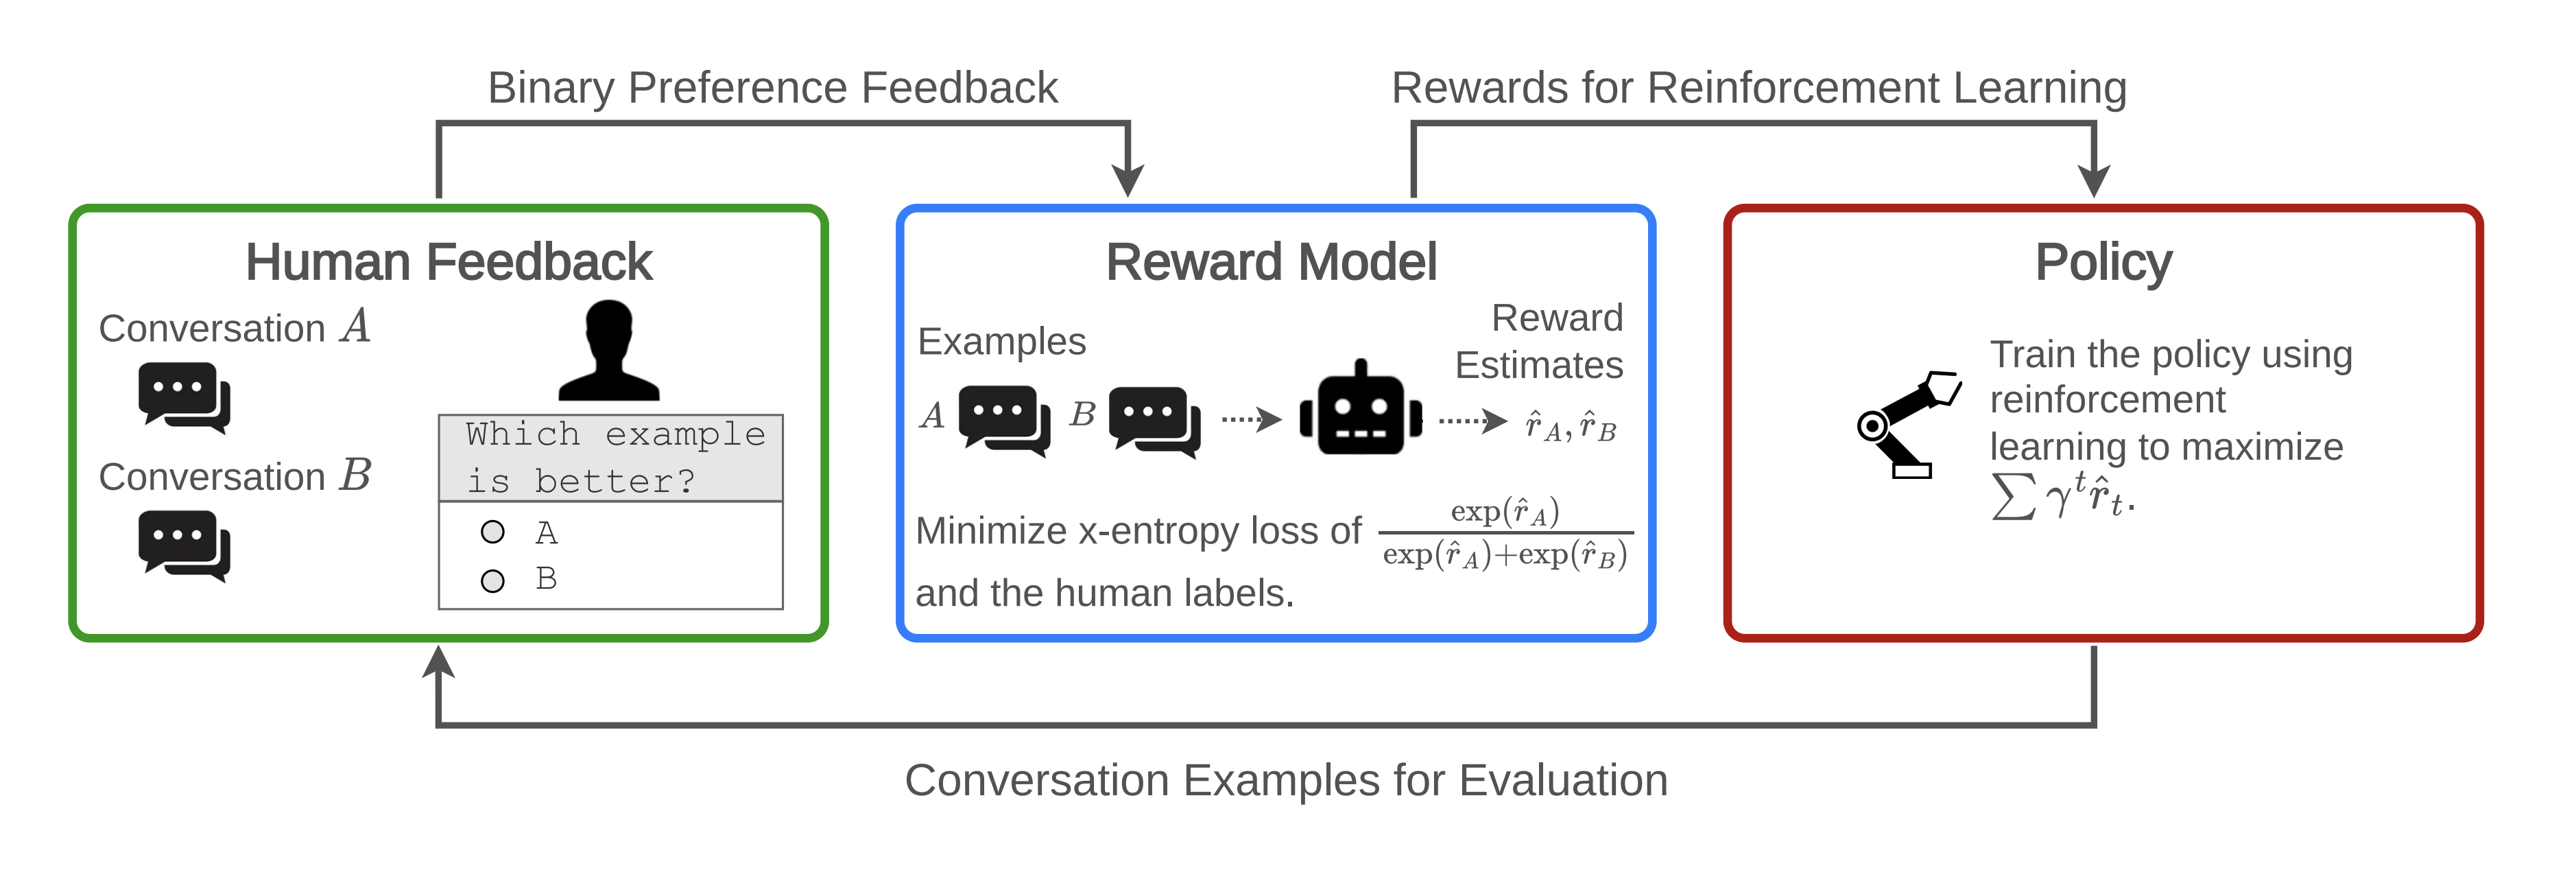
\includegraphics[width=0.99\linewidth]{Figs/rlhf-procedure.png}
    \caption{Illustrated RLHF procedure with a binary feedback provided by the human. From \citet{casper2023open}.}
    \label{fig:rlhf-procedure}
\end{figure}


Generally, $\lambda_p$ is some divergence-based regularizer. The most adopted solution is based on the KL-divergence:

\begin{equation*}
    D_{KL} (P || Q) = \sum_{x \in X} P(x) \log{ \left ( \frac{P(x)}{Q(x)} \right )} = - \sum_{x \in X} P(x) \log{ \left ( \frac{Q(x)}{P(x)} \right )} , 
\end{equation*}

namely a measure of how one probability distribution $P(\theta_{\text{ new}})$ is different from a second, reference probability distribution $Q(\theta)$ with $\theta_{\text{ new}}$ and $\theta$ being respectively the model updated by the PPO procedure and the reference model whose parameters are kept frozen. This measure of statistical distance is employed in this project to prevent model parameters from diverging from the original.

As for the PPO optimization procedure, introduced in 2017 by OpenAI \citep{schulman2017proximal}, appears to be the best balance between optimization performance and ease of implementation. The Proximal Policy Optimization implementation is very close to the original policy gradient but through small changes the algorithm is optimized to outperform the vanilla one in most of the cases.

As previously introduced, given a set of tunable parameters $\theta$, the aim is to update in the direction that yields higher rewards as possible. The policy $\phi_\theta (a | s)$ is defined as stochastic, i.e. the parameters are the only ones that dictate the probability of an action $a$ directly influencing the trajectory $\tau$ defined as a sequence of pairs of states and action $s_1, a_1, ..., s_n, a_n$.

The objective function that PPO aim to optimize is defined as follows:

\begin{equation*}
    J (\theta) = E_{\tau \sim \pi_\theta} R(\tau) = \sum_\tau P(\tau; \theta) R(\tau)
\end{equation*}

By using the stochastic policy, the goal is to sample various actions, recording the corresponding probability and the differences in rewards. Applied to language model generation this means that the model generates a response to the given prompt and then is optimized at each step (if the batch size is equal to 1 sample per time) according to the given reward. To determine the update direction in which the model is optimized, policy gradient methods rely on gradients $\nabla_\theta$, which corresponds to a vector of partial derivatives for the target function (or model). The update is therefore performed according to the function:

\begin{equation*}
    \theta \leftarrow \theta + \alpha \nabla_\theta J(\theta)
\end{equation*}

with $J(\theta)$ embedding the reward function and $\alpha$ being the learning rate. Finding a good learning rate turns out to be a non-trivial problem. In fact, optimization processes of this type tend to over-weight the optimization step by leading the updated model to diverge. For this reason, the proximal policy optimization process, restricts the range within which the policy can be updated. This is performed by a small change to the objective function by clipping the steps according to different cases. The new objective function is defined as follow:

\begin{equation*}
    L^{CLIP}_{\pi_\theta} (\pi_{\theta_k}) = \mathbb{E}_{\tau \sim \pi_\theta} \left[ \sum^T_{t = 0} \left[ \min \left( \rho_t (\pi_\theta, \pi_{\theta_k}) A^{\pi_{\theta_k}}_t , \text{clip}(\rho_t (\pi_\theta, \pi_{\theta_k}), 1 - \epsilon, 1 + \epsilon) A_t^{\pi_{\theta_k}} \right) \right] \right]
\end{equation*}

with the importance sampling ratio $\rho_t$ as a value given by the ratio between the original model $\pi_\theta$ and the updated model $\pi_{\theta_k}$:

\begin{equation*}
    \rho_t (\theta) = \frac{\pi_\theta (a_t | s_t)}{\pi_{\theta_k} (a_t | s_t)} 
\end{equation*}

By analyzing the new objective function, the minimum among all the terms listed (in addition to the clip of some elements) is calculated for conservative issues in terms of optimization, in other words to avoid optimizing strongly toward a direction (new state $s_t$) that may lead to worse future actions ($a_t$). Instead, the $1 - \epsilon$ and $1 + \epsilon$ terms do not depend on the model's parameters $\theta$ but are imposed as boundaries of the region within which the model can move.

In spite of the lack of strong theoretical and mathematical evidence on the convergence of this algorithm \citep{schulman2017trust}, it has been multiply demonstrated that on the empirical level this procedure is generally the fastest and most effective in terms of convergence in the optimization process for reinforcement learning.

Moreover, the structure of the PPO algorithm imposes greater use of the available graphical memory. This happens because two exact copies of the same model in their initial state must be kept in memory, and then only one of these two is updated according to the optimization process. The original version, however, must be held in memory until the end of training. This generally leads to computational complications, but these can be mitigated as explained in later chapters.



\section{Interpretability of Language Models}

Generating human-understandable explanations for the behaviour of AI systems is currently an unsolved problem. Due to their immense complexity, LLMs are generally considered black-box models and this brings with it a number of problems related to the use of LLMs in risky environments where safety, reliability and accountability are necessary features \citep{rudin2019stop}. Although metrics are currently used to measure the effectiveness of models under a large number of different tasks, they still fail to capture all the probable cases of failure that one might have or, better still, fail to explain how a given model makes a decision and what the reasons for it are. The aim of the current research project is to investigate methods of interpretability defined as \textit{post-hoc}, i.e. methods that provide an interpretation of models already trained according to the procedures seen above and that are as agnostic as possible to the model itself.

There are different approaches to interpretability:
\begin{itemize}
    \item Gradient-based: these approaches try to capture the gradient w.r.t. the input by measuring the change of output given an $\epsilon$-change to each input feature \citep{li-etal-2016-visualizing}. This method is defined as functionally grounded but does not always guarantee a trustworthy explanation for non-linear models since the explanation relates to a first-order Taylor approximation.
    \item Perturbation-based: these explanation methods are based on nearby observations $\hat{x}$ of the input $x$. With LIME the model estimates $p(c|\hat{x})$ to fit a logistic regression. The parameters of the logistic regression represent the importance measure \citep{ribeiro-etal-2016-trust}.
    \item Internals-based: For transformer-based models, the attention could provide a good explanation of what the model looks and, consequentially, give importance in order to generate a specific output. By doing so it is possible to look at all the internal layers and parameters to explain the model's behaviour. It is not clear if attention could be considered as an interoperability technique since it does not always provide a good or meaningful output explanation \citep{bibal-etal-2022-attention}.
\end{itemize}

By definition, interpretability techniques aim at explaining a model output to humans \citep{MILLER20191} and, consequentially, they are developed to provide a qualitative explanation. This characteristic leads to difficulties in comparing or quantitatively evaluating any method proposed. Generally, this problem is tackled by checking the meaning of the results found at the human level, and then proceeding with more precise quantitative evaluations. However, there are as yet no standards or guidelines in this regard, leaving the choices to the discretion of the researcher.

Progress in explainability and interpretability could help verify hypotheses about how models make decisions \citep{geiger2023causal} and help in verifying the decision process of the model. A model or process that can be explained would give greater confidence and trust in its decision-making processes, ensuring more than the use of metrics on standard benchmarks the ability not to fail under certain circumstances \citep{jacovi2021formalizing}. Furthermore, an analysis of a model that includes interpretability as a fundamental step could better explain its vulnerabilities. Specifically, looking at model red-teaming attempts \citep{ziegler2022adversarial}, in the case of identifying adversarial inputs it would be possible to generalise the reasons why a given model is prone to fail in that circumstance \citep{rastogi2023supporting, räuker2023transparent}.

Various interpretability techniques could be employed to improve specific aspects of the models, acting on their internal behaviour and improving, for instance, their truthfulness \citep{li2023inferencetime}, changing the factual knowledge they contain \citep{meng2023locating, hernandez2023inspecting} or directly steering their behaviour for certain aspects.

% How interpretability could help:
% Interesting "Interpretability and model editing" paragraph from https://arxiv.org/pdf/2307.15217.pdf
